\chapter{Sorting}

Sorting is simply the process of ordering data in a consistent manner, such as organizing cards, telephone name lists, student name lists, etc.

Each element is usually part of a collection of data called a record. Each record contains a key, which is the value to be sorted, while the remainder of the record consists of satellite data. Here, we have two assumptions: the keys are integers, and the sorting process uses internal memory.

There are several algorithms to sort in \(O(n^2)\), such as insertion sort. There is also an algorithm like Shell sort, which is very simple to code, runs in \(O(n^2)\), and is efficient in practice. Additionally, there are some slightly more complicated sorting algorithms that take \(O(n \log n)\). However, any general-purpose sorting algorithm requires \(\Omega(n \log n)\) comparisons.

\section{Introduction}
\subsection{Preliminaries}
In internal sort, an array containing the elements and an integer containing the number of elements will be passed to the algorithm.

We assume that \(N\), the number of elements passed to our sorting routines, has already been checked and is legal.

We require the existence of the \(<\) and \(>\) operators, which can be used to place a consistent ordering on the input.

\subsection{Operations}
In sorting, there are several operations.

\subsubsection{Permutation}
A permutation of a finite set \(S\) is an ordered sequence of all the elements of \(S\), with each element appearing exactly once. A \(k\)-permutation of \(S\) is an ordered sequence of \(k\) elements of \(S\), with no element appearing more than once in the sequence. 

For example, for \(S = \{a, b, c\}\), there are 6 permutations. For a set of \(n\) elements, there are \(n!\) permutations. 


\subsubsection{Inversion}
An inversion in an array of numbers is any ordered pair \((i, j)\) having the property that \(i < j\) but \(a[i] > a[j]\). 

For example, the input list \(34, 8, 64, 51, 32, 21\) has nine inversions, namely: (34,8), (34,32), (34,21), (64,51), (64,32),
(64,21), (51,32), (51,21) and (32,21). Notice that this is exactly the number of swaps that need to be performed by insertion sort.

\section{Bubble Sort}
\subsection{Operation}
Bubble sort is done by scanning the list from one end to the other, and whenever a pair of adjacent keys is found to be out of order, they are swapped. In this pass, the larger key in the list will have bubbled to the end, but earlier keys may still be out of order.

Bubble sort is probably the easiest algorithm to implement but the most time-consuming of all the algorithms, other than pure random permutation. The basic idea underlying bubble sort is to pass through the file sequentially several times.

In bubble sort, each pass consists of comparing each element in the file with its successor and interchanging the two elements if they are not in proper order. After each pass, the largest element \(x[n - i]\) is in its proper position within the sorting array.

\begin{table}[H]
  \centering
  \begin{tabular}{c|c c c c c c|c}
    \toprule
    Original & 34 & 8 & 64 & 51 & 32 & 21 & Number of Exchanges  \\
    \midrule
    After \(p = 1\) & \textcolor{red}{8} & 34 & 21 & 64 & 51 & 32 & 4  \\
    \midrule
    After \(p = 2\) & \textcolor{red}{8} & \textcolor{red}{21} & 34 & 32 & 64 & 51 & 3  \\
    \midrule
    After \(p = 3\) & \textcolor{red}{8} & \textcolor{red}{21} & \textcolor{red}{32} & 34 & 51 & 64 & 2  \\
    \midrule
    After \(p = 4\) & \textcolor{red}{8} & \textcolor{red}{21} & \textcolor{red}{32} & \textcolor{red}{34} & 51 & 64 & 0  \\
    \midrule
    After \(p = 5\) & \textcolor{red}{8} & \textcolor{red}{21} & \textcolor{red}{32} & \textcolor{red}{34} & \textcolor{red}{51} & 64 & 0  \\
    \midrule
    After \(p = 6\) & \textcolor{red}{8} & \textcolor{red}{21} & \textcolor{red}{32} & \textcolor{red}{34} & \textcolor{red}{51} & \textcolor{red}{64} & 0  \\
    \bottomrule
  \end{tabular}
\end{table}

In this example, for the first pass, it begins from the right. Since \(21 > 32\), it swaps, then we have \(34, 8, 64, 51, 21, 32\). Then we check with \(51\) and \(21\), they are out of order, so we swap again, then we have \(34, 8, 64, 21, 51, 32\). Recursively doing so, we get the sequence \(8, 34, 21, 64, 51, 32\). The sorting will stop when \(p = 6\), which is the number of elements to be sorted.

\subsection{Analysis}
There are in total \(n - 1\) passes and \(n - 1\) comparisons on each pass without the improvement. Thus, the total number of comparisons is \((n - 1)^2 = n^2 - 2n + 1\), which is \(O(n^2)\). 

We can improve this algorithm by stopping the swap when the number of exchanges is equal to 0, i.e., all the elements are in proper order. With the improvement, the sorting will be \((n - 1) + (n - 2) + \cdots + 1 = \frac{n(n + 1)}{2}\), which is also \(O(n^2)\).

The number of interchanges depends on the original order of the file. However, the number of interchanges cannot be greater than the number of comparisons. It is likely that the number of interchanges, rather than the number of comparisons, takes up the most time in the program's execution.

For bubble sort, it requires little additional space. We only need one additional record to hold the temporary value for interchanging and several simple integer variables. It is \(O(n)\) in the case that the file is completely sorted (or almost completely sorted), since only one pass of \(n - 1\) comparisons (and no interchanges) is necessary to establish that the file is sorted.

\section{Insertion Sort}
\subsection{Operation}
Insertion sort again consists of \(n - 1\) passes. For pass \(p = 2\) through \(n\), insertion sort ensures that the elements in positions \(1\) through \(p\) are in sorted order. Insertion sort makes use of the fact that elements in positions \(1\) through \(p - 1\) are already known to be in sorted order.

Initially, \(x[0]\) may be thought of as a sorted file of one element. After each repetition of the loop, the elements \(x[0]\) through \(x[k]\) are in order.

\begin{table}[H]
  \centering
  \begin{tabular}{c|c c c c c c|c}
    \toprule
    Original & 34 & 8 & 64 & 51 & 32 & 21 & Positions Moved  \\
    \midrule
    After \(p = 1\) & \textcolor{red}{34} & 8 & 64 & 51 & 32 & 21 & 0  \\
    \midrule
    After \(p = 2\) & \textcolor{red}{8} & \textcolor{red}{34} & 64 & 51 & 32 & 21 & 1  \\
    \midrule
    After \(p = 3\) & \textcolor{red}{8} & \textcolor{red}{34} & \textcolor{red}{64} & 51 & 32 & 21 & 0  \\
    \midrule
    After \(p = 4\) & \textcolor{red}{8} & \textcolor{red}{34} & \textcolor{red}{51} & \textcolor{red}{64} & 32 & 21 & 1  \\
    \midrule
    After \(p = 5\) & \textcolor{red}{8} & \textcolor{red}{32} & \textcolor{red}{34} & \textcolor{red}{51} & \textcolor{red}{64} & 21 & 3 \\
    \midrule
    After \(p = 6\) & \textcolor{red}{8} & \textcolor{red}{21} & \textcolor{red}{32} & \textcolor{red}{34} & \textcolor{red}{51} & \textcolor{red}{64} & 4 \\
    \bottomrule
  \end{tabular}
\end{table}

In this example, for the first pass, we treat 34 as sorted, thus no move is needed. Then we 'insert' 8, since it is smaller than 34, it is moved before 34. By doing so recursively, we can have a sorted list. 

\subsection{Analysis}
The simple insertion sort may be viewed as a general selection sort in which the priority queue is implemented as an ordered array. Only the preprocessing phase of inserting the elements into the priority queue is necessary. Once the elements have been inserted, they are already sorted, so no selection is necessary.

If the initial file is sorted, only one comparison is made on each pass, so the sort is \(O(n)\). However, if the file is initially sorted in reverse order, the sort is \(O(n^2)\), since the total number of comparisons is \((n - 1) + (n - 2) + \cdots + 2 + 1 = \frac{(n - 1)n}{2}\), which is still \(O(n^2)\).

The simple insertion sort is still usually better than the bubble sort. The closer the file is to sorted order, the more efficient the simple insertion sort becomes. The average number of comparisons in the simple insertion sort is also \(O(n^2)\), considering all possible permutations of the input array.

The space requirements for the sort consist of only one temporary variable \( y \). Insertion sort makes \( O(n^2) \) comparisons of keys and \( O(n^2) \) movements of entries. It makes \(\frac{n^2}{4} + O(n)\) comparisons of keys and movements of entries when sorting a list of length \( n \) in random order. 

To improve, we can use a binary search. This reduces the total number of comparisons from \( O(n^2) \) to \( O(n \log n) \). However, the moving operation still requires \( O(n^2) \) time. So the binary search does not significantly improve the overall time requirement. 

We can also improve the algorithm by using list insertion. This reduces the time required for insertion but not the time required for searching for the proper position. The average number of inversions in an array of \( n \) distinct numbers is \( \frac{n(n-1)}{4} \). 

For any list \( L \) of numbers, consider \( L_r \), which is the list in reversed order. Consider any pair of two numbers in the list \( (x, y) \) with \( y > x \). In exactly one of \( L \) and \( L_r \), this ordered pair represents an inversion. The total number of these pairs in a list \( L \) and its reverse \( L_r \) is \( \frac{n(n-1)}{2} \). On average, it is half of the above. 

Any algorithm that sorts by exchanging adjacent elements requires \( \Omega(n^2) \) time on average. The average number of inversions is initially \( \Omega(n^2) \), and since each swap removes only one inversion, \( \Omega(n^2) \) swaps are required.

\section{Selection Sort}
\subsection{Operation}
Selection sort is also called Straight Selection or Push-Down Sort. A selection sort is one in which successive elements are selected in order and placed into their proper sorted positions. The elements of the input may have to be preprocessed to make the ordered selection possible. 

At the first stage, one scans the list to find the entry that comes last in the order. This entry is then interchanged with the entry in the last position. By omitting the last entry, we can repeat the process on the shorter list.

\begin{table}[H]
  \centering
  \begin{tabular}{c|c c c c c c|c}
    \toprule
    Original & 34 & 8 & 64 & 51 & 32 & 21 & Positions Moved  \\
    \midrule
    After \(p = 1\) & 34 & \textcolor{cyan}{8} & 64 & 51 & 32 & 21 & 1  \\
    \midrule
    After \(p = 2\) & \textcolor{red}{8} & 34 & 64 & 51 & 32 & \textcolor{cyan}{21} & 4  \\
    \midrule
    After \(p = 3\) & \textcolor{red}{8} & \textcolor{red}{21} & 64 & 51 & \textcolor{cyan}{32} & 34 & 2  \\
    \midrule
    After \(p = 4\) & \textcolor{red}{8} & \textcolor{red}{21} & \textcolor{red}{32} & 51 & 64 & \textcolor{cyan}{34} & 2  \\
    \midrule
    After \(p = 5\) & \textcolor{red}{8} & \textcolor{red}{21} & \textcolor{red}{32} & \textcolor{red}{34} & 64 & \textcolor{cyan}{51} & 1 \\
    \midrule
    After \(p = 6\) & \textcolor{red}{8} & \textcolor{red}{21} & \textcolor{red}{32} & \textcolor{red}{34} & \textcolor{red}{51} & \textcolor{cyan}{64} & 0 \\
    \bottomrule
  \end{tabular}
\end{table}

Here, we scan from the first element that comes in the order, which will give us the same sorted list. In the first scan, 8 is found to be the smallest element, so we swap it with the element in the first position. Then, 21 is found to be the second smallest element, so it is swapped with the element in the second position. By doing so recursively, we obtain a sorted list.

\subsection{Analysis}
Here we can do a simple comparison: 

\begin{table}[H]
  \centering
  \begin{tabular}{c|c|c}
      \toprule
       & Selection & Insertion (average)  \\
    \midrule
      Assignments of entries & \(3n + O(1)\) & \(0.25n^2 + O(n)\)  \\
      Comparisons of keys & \(0.5n^2 + O(n)\) & \(0.25n^2 + O(n)\)  \\
      \bottomrule
  \end{tabular}
\end{table}

The algorithm consists entirely of a selection phase in which the largest of the remaining elements \(L\) is repeatedly placed in its proper position \(i\) at the end of the array. To do so, \(L\) is interchanged with the element \(x[i]\). The initial \(n\)-element priority queue is reduced by one element after each selection.

The first pass makes \(n - 1\) comparisons, the second pass makes \(n - 2\), and so on. Therefore, the total number of comparisons is \(\frac{n(n - 1)}{2} = O(n^2)\).

The number of interchanges is always \(n - 1\) unless a test is added to prevent the interchanging of an element with itself.

There is little additional storage required except to hold a few temporary variables. The sort may be categorized as \(O(n^2)\), although it is faster than bubble sort. There is no improvement if the input file is completely sorted or unsorted, since the testing proceeds to completion without regard to the makeup of the file.

\section{Shell Sort}
\subsection{Operation}
Shell sort is also called Diminishing Increment Sort. Selection sort moves the entries very efficiently, but there are many redundant comparisons. Also, even in the best case, insertion sort does the minimum number of comparisons, but it is inefficient in moving entries only one place at a time.

If we modify the comparison method so that it first compares keys far apart, then it could sort the entries that are far apart. Afterward, the entries closer together would be sorted, and finally, the increment between keys being compared would be reduced to 1, ensuring that the list is completely in order. This is what we call shell sort.

One requirement that is intuitively clear is that the elements of the increment sequence should be relatively prime. This guarantees that successive iterations intermingle subfiles so that the entire file is indeed almost sorted when the increment equals 1 in the last iteration.

\begin{table}[H]
  \centering
  \begin{tabular}{c|c c c c c c c c c c c c c}
      \toprule
      Original & 81 & 94 & 11 & 96 & 12 & 35 & 17 & 95 & 28 & 58 & 41 & 75 & 15  \\
    \midrule
      After 5-sort & \colorbox{Apricot}{35} & \colorbox{CornflowerBlue}{17} & \colorbox{Lavender}{11} & \colorbox{yellow}{28} & \colorbox{lime}{12} & \colorbox{Apricot}{41} & \colorbox{CornflowerBlue}{75} & \colorbox{Lavender}{15} & \colorbox{yellow}{96} & \colorbox{lime}{58} & \colorbox{Apricot}{81} & \colorbox{CornflowerBlue}{94} & \colorbox{Lavender}{95}  \\
      After 3-sort & \colorbox{Apricot}{28} & \colorbox{CornflowerBlue}{12} & \colorbox{Lavender}{11} & \colorbox{Apricot}{35} & \colorbox{CornflowerBlue}{15} & \colorbox{Lavender}{41} & \colorbox{Apricot}{58} & \colorbox{CornflowerBlue}{17} & \colorbox{Lavender}{94} & \colorbox{Apricot}{75} & \colorbox{CornflowerBlue}{81} & \colorbox{Lavender}{96} & \colorbox{Apricot}{95}  \\
      After 2-sort & \colorbox{Apricot}{11} & \colorbox{CornflowerBlue}{12} & \colorbox{Apricot}{15} & \colorbox{CornflowerBlue}{17} & \colorbox{Apricot}{28} & \colorbox{CornflowerBlue}{35} & \colorbox{Apricot}{58} & \colorbox{CornflowerBlue}{41} & \colorbox{Apricot}{81} & \colorbox{CornflowerBlue}{75} & \colorbox{Apricot}{94} & \colorbox{CornflowerBlue}{96} & \colorbox{Apricot}{95}  \\
      After 1-sort & \colorbox{Apricot}{11} & \colorbox{Apricot}{12} & \colorbox{Apricot}{15} & \colorbox{Apricot}{17} & \colorbox{Apricot}{28} & \colorbox{Apricot}{35} & \colorbox{Apricot}{41} & \colorbox{Apricot}{58} & \colorbox{Apricot}{75} & \colorbox{Apricot}{81} & \colorbox{Apricot}{94} & \colorbox{Apricot}{95} & \colorbox{Apricot}{96}  \\
      \bottomrule
  \end{tabular}
\end{table}

At first, we perform sorting with an increment of 4, so elements in positions 1, 6, and 11 are sorted; 2, 7, and 12 are sorted; and 3, 8, and 13 are sorted. By doing so recursively, we obtain a sorted list. 

Since the first increment used by Shell sort is large, the individual subfiles are quite small, making the simple insertion sorts on those subfiles fairly fast. Each sort of a subfile causes the entire file to become more nearly sorted. Although successive passes of Shell sort use smaller increments and therefore deal with larger subfiles, those subfiles are almost sorted due to the actions of previous passes. Thus, the insertion sorts on those subfiles are also quite efficient. 

\subsection{Analysis}
If a file is partially sorted using an increment \(k\) and is subsequently partially sorted using an increment \(j\), the file remains partially sorted on the increment \(k\). Hence, subsequent partial sorts do not disturb the earlier ones. 

The analysis of Shell sort is difficult at best. Empirical studies on Shell sort show that when \( n \) is large, the running time is in the range of \( n^{1.25} \) to \( 1.6n^{1.25} \). It has been shown that the order of Shell sort can be approximated by \( O(n (\log n)^2) \) if an appropriate sequence of increments is used. For other series of increments, the running time can be proven to be \( O(n^{1.25}) \).

Empirical data indicate that the running time is of the form \( a \times n^b \), where \( a \) is between 1.1 and 1.7, and \(b\) is approximately 1.26, or of the form \( c \times n(\log n)^2 - d \times n \times \log n \), where \( c \) is approximately 0.3 and \( d \) is between 1.2 and 1.75. 

In general, Shell sort is recommended for moderately sized files of several hundred elements.

Knuth recommends choosing increments as follows:

- Define a function \(h\) recursively so that \(h(1) = 1\) and \(h(i + 1) = 3 \times h(i) + 1\).

- Let \(x\) be the smallest integer such that \(h(x) \geq n\), and set \texttt{numinc}, the number of increments, to \(x - 2\) and \texttt{incrmnts[i]} to \(h(\texttt{numinc} - i + 1)\) for \(i\) from 1 to \texttt{numinc}.

\section{Heap Sort}
Heap sort is similar to an AVL tree. Priority queues can be used to sort in \(O(n \log n)\) time, which gives the best big-O running time we have seen so far.

To perform heap sort, we build a max binary heap of \(n\) elements. This stage takes \(O(n)\) time. We then perform \(n\) \texttt{delete\_max} operations. The elements leave the heap, smallest first, in sorted order. By recording these elements in a second array and then copying the array back, we sort the \(n\) elements. Since each \texttt{delete\_max} operation takes \(O(\log n)\) time, the total running time is \(O(n \log n)\).

The main problem with this algorithm is that it uses an extra array. Thus, the memory requirement is doubled. To address this, we use the last cell for storing the array. Since after each \texttt{delete\_max}, the heap shrinks by 1, the cell that was last in the heap can be used to store the element that was just deleted.

\begin{center}
\begin{minipage}{0.32\textwidth}
  \begin{figure}[H]
    \centering
    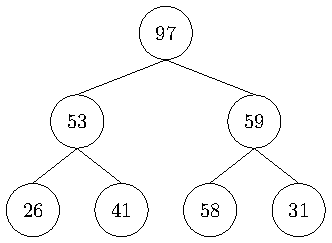
\includegraphics[width=\textwidth]{Figure/HeapSort1.pdf}
    \caption*{97, 53, 59, 26, 41, 58, 31}
  \end{figure}
\end{minipage}
\begin{minipage}{0.32\textwidth}
  \begin{figure}[H]
    \centering
    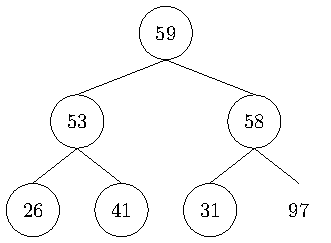
\includegraphics[width=\textwidth]{Figure/HeapSort2.pdf}
    \caption*{53, 59, 26, 41, 58, 31, 97}
  \end{figure}
\end{minipage}
\begin{minipage}{0.32\textwidth}
  \begin{figure}[H]
    \centering
    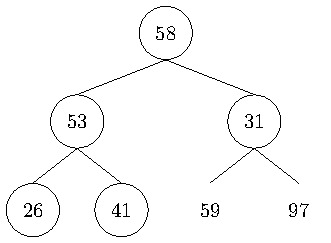
\includegraphics[width=\textwidth]{Figure/HeapSort3.pdf}
    \caption*{53, 26, 41, 58, 31, 59, 97}
  \end{figure}
\end{minipage}
\end{center}

\begin{center}
\begin{minipage}{0.32\textwidth}
  \begin{figure}[H]
    \centering
    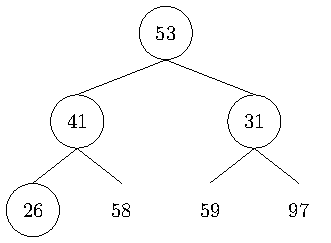
\includegraphics[width=\textwidth]{Figure/HeapSort4.pdf}
    \caption*{53, 26, 41, 31, 58, 59, 97}
  \end{figure}
\end{minipage}
\begin{minipage}{0.32\textwidth}
  \begin{figure}[H]
    \centering
    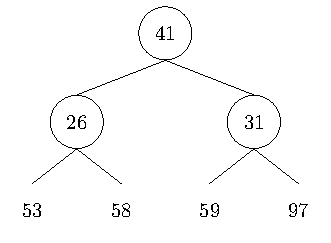
\includegraphics[width=\textwidth]{Figure/HeapSort5.pdf}
    \caption*{26, 41, 31, 53, 58, 59, 97}
  \end{figure}
\end{minipage}
\begin{minipage}{0.32\textwidth}
  \begin{figure}[H]
    \centering
    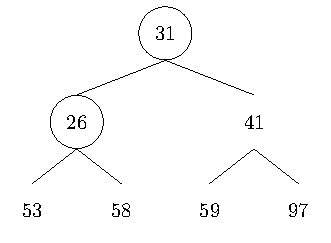
\includegraphics[width=\textwidth]{Figure/HeapSort6.pdf}
    \caption*{26, 31, 41, 53, 58, 59, 97}
  \end{figure}
\end{minipage}
\end{center}

\begin{center}
\begin{minipage}{0.32\textwidth}
  \begin{figure}[H]
    \centering
    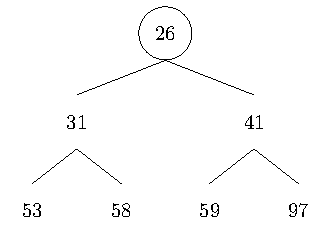
\includegraphics[width=\textwidth]{Figure/HeapSort7.pdf}
    \caption*{26, 31, 41, 53, 58, 59, 97}
  \end{figure}
\end{minipage}
\begin{minipage}{0.32\textwidth}
  \begin{figure}[H]
    \centering
    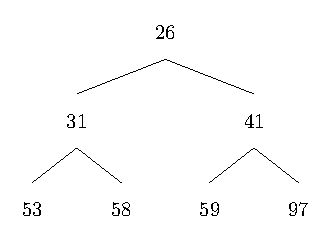
\includegraphics[width=\textwidth]{Figure/HeapSort8.pdf}
    \caption*{97, 53, 59, 26, 41, 58, 31}
  \end{figure}
\end{minipage}
\end{center}

Here, we first remove the largest key, which is 97 in this case, and rearrange the heap. Then, we place 97 in the hole left empty due to the deletion. By doing so recursively, we obtain a sorted list.

\section{Merge Sort}
\subsection{Operation}
Merge sort is an excellent method for external sorting, which is used for problems where the data are kept on disks or magnetic tapes, rather than in high-speed memory (RAM).

\begin{minipage}{0.4\textwidth}
This algorithm is a classic divide-and-conquer strategy. The problem is divided into smaller sub-problems and solved recursively. The conquering phase consists of patching together the solutions to the sub-problems. Divide-and-conquer is a very powerful use of recursion that we will see many times. \\[3pt]
Comparisons of keys are done at only one place in the entire merge sort procedure. This place is within the main loop of the merge procedure. After each comparison, one of the two nodes is sent to the output list. Hence, the number of comparisons certainly cannot exceed the number of nodes being merged. \\[3pt]
As shown on the right, we divide the array into two halves recursively until it cannot be further divided. Then, we perform merge sort recursively. For the first merge sort, since there is only one element, it is already sorted. Then, we merge two elements and sort them in order. By doing this recursively, we obtain the sorted list. 
\end{minipage}
\begin{minipage}{0.6\textwidth}
  \begin{figure}[H]
    \centering
    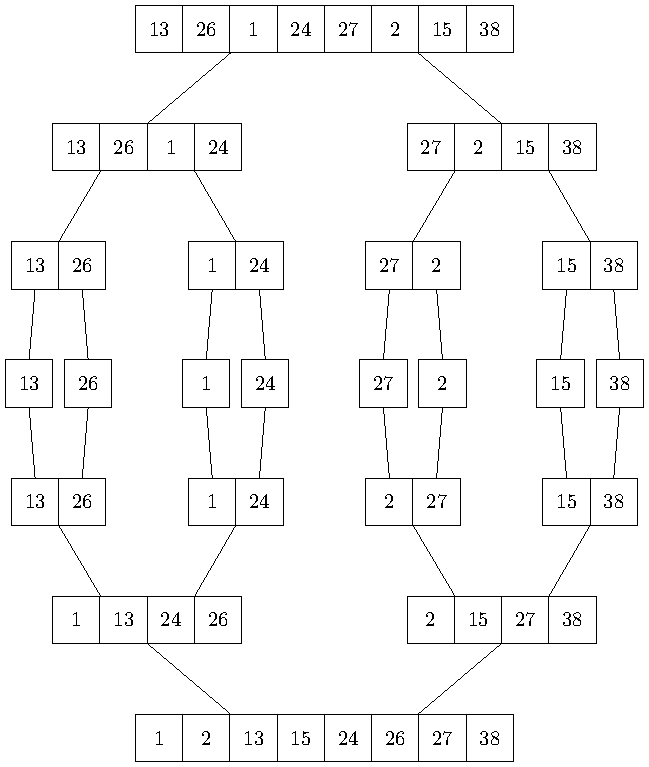
\includegraphics[width=0.8\textwidth]{Figure/MergeSort.pdf}
    \caption*{Merge Sort}
  \end{figure}
\end{minipage}

\subsection{Analysis}
It is clear from the tree that the total length of the lists on each level is precisely \(n\), the total number of entries. In other words, every entry is treated in exactly one merge on each level. Hence, the total number of comparisons done on each level cannot exceed \(n\). The number of levels, excluding the leaves for which no merges are done, is \(\lceil \log n \rceil\), the ceiling of \(\log n\). Therefore, the total number of comparisons of keys done by merge sort on a list of \(n\) entries is no more than \(n \log n\), rounded up.

\begin{proof}
\[
\begin{aligned}
  T(1) &= 1 \\
  T(n) &= 2T(\frac{n}{2}) + n \\
  \frac{T(n)}{n} &= \frac{T(\frac{n}{2})}{\frac{n}{2}} + 1 \\
  \frac{T(\frac{n}{2})}{\frac{n}{2}} &= \frac{T(\frac{n}{4})}{\frac{n}{4}} + 1 \\
  &\vdots \\
  \frac{T(2)}{2} &= \frac{T(1)}{1} + 1 \\
  \frac{T(n)}{n} &= \frac{T(1)}{1} + \log n \\
  T(n) &= n\log n + n = O(n\log n)
\end{aligned}
\]
\end{proof}

\section{Quick Sort}


\section{Radix Sort}
